%!TEX root = ../main.tex
\chapter{Literature Review}
\label{chap:litReview}

For this project I will need to research three key areas: the psychological aspects of motivation, particularly in children; gamification; video game and mobile application development.
Research will need to be made specifically into how I can not only encourage children to use the app, but how I can best ensure that the app is both fun - to encourage continued play - and beneficial to the child's motivation skills.
Other important research areas will be what software development methodology will be most beneficial to me as a lone developer, and what methods of testing are best suited towards ensuring a high quality deliverable.

\section{Gamification}
\subsection{Defining Gamification}
A definition of gamification is offered by \citet[p.6]{Deterding:2011:GDE:2181037.2181040} as ``The use of design elements for games in non-game contexts''. 
A game design element in this case is referred to as the characteristics of a game that appear in most games, are readily associated with games and are found to play a significant role in games.
With this definition, it is necessary to identify the game design elements that will be included in the application. 

In this paper, Deterding also highlights the fact that Gamification refers specifically to using game elements in a non-game application, rather than using full-fledged games.
Therefore, by this strict definition, it is important to draw the distinction between a game application built to incorporate real-life rewards and a motivational application built to incorporate game-based elements.

\citet[p.5]{huotari2011gamification} have also provided an alternative definition for gamification, stating that it is ``service packaging where a core service is enhanced by a rules-based service system that provides feedback and interaction mechanisms to the user with an aim to facilitate and support the users’ overall value creation.''

\subsection{Rewards and Punishments}
In an experiment by \cite{Filsecker2014136}, children were separated into two groups: a public recognition (PR) group where the children's `badges' were recorded on a prominently placed leaderboard in a room where others can see, and a non-public recognition (NPR) group.
The children were then given an educational game called Taiga which would ask them to pose a hypothesis about decreasing numbers of fish in a pond, and then perform experiments to justify or disprove the hypothesis.

It was found that students achieved a statistically significant increase in understanding and performance of topics in the PR group when compared to the NPR group.
Taiga had a variety of educational content embedded within the game that the users can access, and tracked which ones the children had checked during the tasks to determine whether the children were motivated to access more of these. 
However, it was unexpectedly also found that the PR group did not access any more of these educational materials than the NPR group, which - given the previous findings - could insinuate that the increased performance was derived from increased confidence in the subject matter. 

Furthermore, the badges awarded by Taiga are synonymous with the common game design element of `Achievements', which are awarded to the user after a certain set of requirements have been met, e.g. ``Achievement Unlocked - Complete 10 Quests'', and are a useful tool for encouraging users to complete many short tasks in order to earn a long-term reward \cite{hamari2011framework}.

A common issue with rewards in education is that `extrinsic' rewards - i.e. rewards not relating to the activity they are awarded for - ultimately end up undermining the child's attention and motivation from the intrinsic learning activity once the rewards are removed \citep{deci2001extrinsic,ACP:ACP2350090502}.
It can be derived,  therefore, that the rewards are less useful as long-term motivation for children, especially if the rewards cease to be given.
However, \cite{cameron2001negative} highlights that this effect only occurs with children who had high initial interest in the task at hand. 
For example, rewarding a child for performing in his favourite sport only serves to undermine their original interest in the sport.
An explanation for this effect might be that by offering the reward, the child's goal for playing the sport has shifted from `I want to play Rugby' to `I want to earn this reward offered for playing Rugby'.
This means that once the reward has stopped, the incentive for playing has also stopped.

During a meta-analysis of studies into rewards in education, \cite{deci2001extrinsic} also found that unexpected rewards had the least negative impact and highest positive effect for children's long term attention to a task. 
This could mean that it would be beneficial to include an element of randomness to the rewards for completing a task, such as a random chance of earning an increased reward or an extra, but separate, reward.
\cite{king2010video} lists a variety of different reward structures in video games, such as in-game currency, experience points, levelling up and `rare-item' rewards. 
In role-playing games (RPGs), quests often have these key reward structures and, therefore, are established to work suitably well for this project.

\section{Game Design}
\subsection{Game Design Elements}
As previously mentioned, it is important to specify which game design elements I will choose to use in my application.
In the book `100 Elements of Game Design' \citep{despain2012100}, it mentions several useful elements to use.

\cite{Deterding:2011:GDE:2181037.2181040} separated game design elements into five different levels as shown in appendix \ref{appendix:deterdinglevels}.
The key elements I will focus on in my research are `Game interface design patterns', which are common components in games that are not specifically `played with' themselves, but run alongside a game to offer more feedback or fun within the application.
This includes elements such as badges/achievements, leader-boards, levels and experience points. 

\subsubsection{Achievements}
\citet[p.94]{Montola:2009:AGA:1621841.1621859} performed an experiment to determine the usefulness of achievements within a non-game application by adding them to an image hosting and sharing website.
Achievements are defined in this paper as ``optional sub-goals in a secondary reward system'' and are described as being separate to the core game system.
These sub-goals do not affect the progress of the player and should be seen as more of a meta-game, rather than being integral to the game itself.
Concerns were initially raised that adding achievements to non-game applications would encourage unproductive or unintended behaviours by users. An example of this would be an achievement on a forum for making 1000 posts. This may inadvertently motivate users to make a large amount of low-effort or spam posts, reducing the overall quality of the forum.
However, \cite{Montola:2009:AGA:1621841.1621859} noted that some users appreciated the changes and found the achievements to be motivating.
Achievement features are one of the most commonly implemented game design patterns in gamification \citep{hamari2011framework}. 

\subsubsection{Feedback Loops}
A positive feedback loop involves the player becoming more powerful throughout the game, which, in turn, makes things easier to complete. This means they can complete more quests and become more powerful even quicker.
Whilst this sounds like a good element to the game, it is important that developers avoid allowing this to destabilise the game, by making quests - and therefore the game - trivial.
The project artefact will be largely unaffected by this, because quests are completed in the real world and are not tied into the in-game character's power. 
However, if I seek to include an element of competitiveness into the game by allowing users to `battle' each other, it is important to take steps to avoid players becoming so powerful that the battles are no longer enjoyable.

\section{Smartphone Applications}
\subsection{Android vs. iOS}
When planning the development of a mobile application, it must be considered which platform is best to target. 

\subsubsection{Market Share}
Appendix \ref{appendix:worldwidesmartphonemarketshare} clearly shows Android's stronghold over the global market share, holding over 70\% of units shipped since Q3 of 2012. 
Appendix \ref{appendix:uksmartphonemarketshare} also shows an Android dominance in the UK market specifically. 
In these findings, however, the hold over the market is less strong - at 57\% in 2014 and 52\% in 2015 - and shows a downward trend in the market share of Android.

\subsubsection{Fragmentation}
A common issue with developing for mobile phones is that many people do not (or cannot) update their devices to the latest versions.
This problem is referred to as `Fragmentation' and is particularly problematic in Android, as shown in appendix \ref{appendix:sdkmarketshare}.
Despite being released in October of 2015, the latest Android version of Marshmallow is still at less than 2.5\% adoption rate. 
This is primarily due to software updates being held back by network carrier locked phones and phones falling out of support.

As Android phones are manufactured by a number of different companies, there is less standardisation between available handsets. 
\cite{uniqueandroiddevices} reported that it detected nearly 24,100 distinct devices that downloaded its app in 2015, showing just how much of a problem fragmentation could pose to Android development.
This also leads to concerns about the variety of screen sizes in these devices, as apps will have to be designed and maintained to support myriad phones. 
However, \cite{androidscreenfragmentation} shows that, due to the similarities of resolutions between these phones, there are only four key aspect ratios that need to be managed within Android. This is due to the operating systems' implementation of scaling.

\subsection{Human-Computer Interaction}
Human-Computer Interaction (HCI) is the study and analysis of how an end user interacts with a device, this can also be described as the usability of a system.
\citet[p.118]{nielsen1994usability} states that ``The actual effectiveness of a system is achieved when there is an appropriate balance between functionality and usability''.
This means that in order to create a truly functional system there must be some focus on it's ease of use.
HCI also analyses the context in which a user may interact with a system and when designing a mobile application it is important to note the differences in the environment between a user using a desktop PC application and a mobile phone application.
Such as how a user may be involved in other tasks whilst using a mobile app, compared to a traditional PC where much of the user's focus is on directed at the computer \citep{kristoffersen1999making}. 

\section{Development}
\subsection{Waterfall}
The waterfall design methodology is a sequential design process focused on the project progressing to each stage of development one at a time. 
For example, the design stage of the software would not take place until all requirements have been gathered and finalised.
Waterfall is considered to be a very structured methodology and is particularly useful when the requirements are well known and are fixed before the project begins and when the project and the technologies are well understood.

However, due to the rigidity of the Waterfall method, particularly around the planning phase, it is easy for mistakes made early on in the software development life cycle to become embedded within the project and be carried forward to later stages.
For example, if a mistake is made during the requirements-gathering phase and is not noticed until a later phase of the project, it will be very costly to change.
This approach means that risks to the project can be left unnoticed until it is too late in the project to change \citep{kruchten2001waterfall}. % this senstence reads "it is too late in the project to change Kruchten." But I want to change Kruchten!

\subsection{Agile}
The Agile design methodology is a well established and iterative design process that involves regularly moving between stages of the project in a non-sequential manner. 
Agile is very adaptable and allows for more flexibility to the software when design issues arise by not finalising the specification for the whole project too early.
By iteratively planning the design of the project, it allows for quick responses to feed back and if one part of the project is changed, it should have minimal effect on the rest of the project stages. 

\begin{figure}[ht]
	\centering
	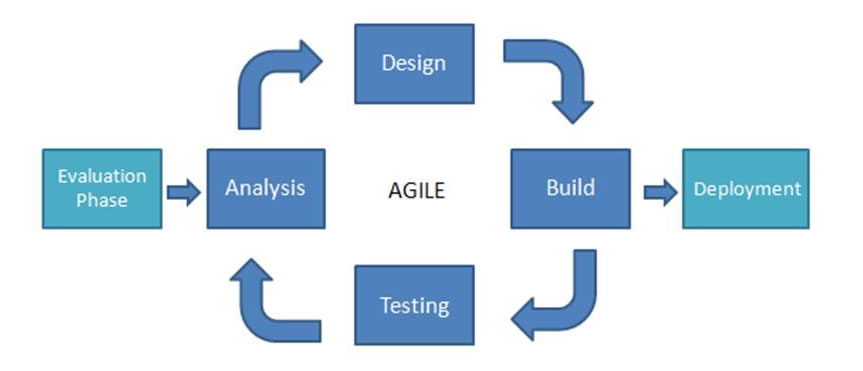
\includegraphics[scale=0.4]{images/Agile_Image.jpg}
	\caption{Iterative Agile Development Process}
	\label{fig:agile}
\end{figure}

Agile dictates that testing should take place regularly throughout the project and by iteratively testing the software at various stages in the life cycle, it gives the developer more chances to catch bugs early.
Under agile, defects discovered in software should be fixed as soon as possible after discovery \citep{beck2001agile}.
In a study by \cite{talby2006}, it was found that by following this practice, defects took less time to fix than without.
This may be due to the fact that the developed features are still fresh in the mind of the developer, who is therefore more readily able to see the problem area and fix it.
The study also found that by keeping the bugs fixed and the code base stable throughout the project, it actually made the development phases of the project faster.

Furthermore, agile testing helps minimise the risks of bugs making it into the final artefact. 
If there was a single testing phase at the end of the project, it is possible that there would be more bugs than anticipated and that the developers would run out of time to properly fix them all. 
By using agile testing, this risk is minimised by allowing developers to better manage the time of testing, as the development of certain low priority features can be delayed or cancelled earlier in the project to allow more time to ensure a quality end product.

\subsection{Test-Driven Development}
As mentioned previously, one of the key principles of agile development is regular and iterative testing throughout the software development life cycle.
This means that test-driven development (TDD) could be a useful tool to work alongside it.
A key factor of TDD is planning out the testing phases of the project before the development of that phase begins.
The workflow of TDD is as follows \citep{Beck:2002:TDD:579193}:
\begin{enumerate}
	\item Add a test that tests the new feature works
	\item Run all tests and see the new one fail
	\item Write the code that makes the test pass
	\item Run all tests and see them all succeed
	\item Refactor the code and tests to remove duplication
	\item Repeat
\end{enumerate}

A study by \cite{George:2003:IIT:952532.952753} found that developers following TDD produced higher quality code which passed 18\% more functional tests.

A software group at IBM made the drastic change from an ad-hoc approach to testing to a TDD-based workflow. They found that, at the cost of a small drop in productivity, their defect rate was reduced by 50\%, the code quality was generally increased and was more flexible to changes, and that morale was generally higher \citep{IBMTDD}. 
The paper also considered that the drop in productivity may well have been down to the change to an unfamiliar system rather than an inherent flaw in TDD, though - due to the increased time writing, preparing and running tests - it is not unusual that TDD might have this effect.